\section{Evaluation}\label{chapter.discussion}
\thispagestyle{plain}

This chapter starts by introducing a collection of test sets used to measure the performance of the allocations mechanism \emph{Opti-X} through experiments, and compare it to the performance of OR-X on the same collection. The results are evaluated and discussed, followed by an assessment of factors that may threat the validity of the results obtained in the experimental phase. \toolname \space is then discussed and evaluated as a whole, before the chapter rounds off by discussing the return on the investment put into this project.

\comment{
\subsection{Research Questions?}
Look at Mortens report for inspiration. Or maybe not?
}

\subsection{Experimental Evaluation}
%\improvement[inline]{TODO}
\comment{- Present test data, run experimental tests and create tables and charts, include a second version of or-x that runs without interruption in order to compare Opti-X and OR-X to the actual optimal overall running duration!}

The collection of test data is made up of four sub-collections, each designed to measure the performance of the allocation mechanism with a particular number of tests and machines available. Each of these sub-collections consist of three test sets; one in which every test can be executed on every machine, one where the tests can only be executed on a small selection of the machines, and one where the number of machines each test can be executed on varies and is determined at random.

\begin{table}[h]
  \begin{tabular}{cccc}
    \hline
    \textbf{Test Set} & \textbf{\# of Tests} & \textbf{\# of Machines} & \textbf{\# of Executable On}\\
    \hline
    $ts_{1}$   &  1000        &   100        &   100\\
    $ts_{2}$   &  --- " ---   &   --- " ---  &   10\\
    $ts_{3}$   &  --- " ---   &   --- " ---  &   \emph{Random}\\
    \hline
    $ts_{4}$   &  --- " ---   &   10          &   10\\
    $ts_{5}$   &  --- " ---   &   --- " ---   &   5\\
    $ts_{6}$   &  --- " ---   &   --- " ---   &   \emph{Random}\\
    \hline
    $ts_{7}$   &   200        &   50          &   50\\
    $ts_{8}$   &   --- " ---  &   --- " ---   &   10\\
    $ts_{9}$   &   --- " ---  &   --- " ---   &   \emph{Random}\\
    \hline
    $ts_{10}$  &   --- " ---  &   10          &   10\\
    $ts_{11}$  &   --- " ---  &   --- " ---   &   5\\
    $ts_{12}$  &   --- " ---  &   --- " ---   &   \emph{Random}\\
    \hline
  \end{tabular}
  \centering
  \caption{Test Data}
  \label{test_data}
\end{table}

Table \ref{test_data} shows the details of each test set in the collection. The test data is randomly generated; only the number of tests, test machines and how many machines each test should be executable on was specified upon generation. Each test was assigned a duration between 30 and 120 seconds, and a set of machines on which they were executable on, both generated at random. The collection of test sets are designed to create a realistic environment, albeit somewhat amplified, while retaining purpose. Larger test sets than $ts_1$ through $ts_3$ would not be very meaningful, as 1000 tests and 100 test machines are very large numbers in this context, and are not likely to be exceeded any time soon.

The test sets, located in \emph{optirun/controller/test\_data/input}, are stored as JSON objects in files with the naming convention \emph{{test\_set\_x.json}}, where

\begin{table}[h]
    \centering
  \footnotesize
  \begin{tabular}{|c|ccc|ccc|}
    \hline
    &  \multicolumn{3}{c|}{\textbf{\large{Opti-X}}} & \multicolumn{3}{c|}{\textbf{\large{OR-X}}}\\
    \emph{Test Set} & \emph{$T_s$} & \emph{$T_e$} & \emph{$T_t$} & \emph{$T_s$} & \emph{$T_e$} & \emph{$T_t$}\\
    \hline
    $ts_{1}$   &   $30.04s$    &   $777.00s$     &   $\mathbf{807.04s}$     &   $34.93s$    &   $1153.00s$   &   $\mathbf{1187.93s}$ \\
    $ts_{2}$   &   $8.66s$     &   $752.00s$     &   $\mathbf{760.66s}$     &   $34.25s$    &   $1224.00s$   &   $\mathbf{1258.25s}$ \\
    $ts_{3}$   &   $0.29s$     &   $867.00s$     &   $\mathbf{867.29s}$     &   $34.44s$    &   $1172.00s$   &   $\mathbf{1206.44s}$ \\
    \hline
    $ts_{4}$   &   $0.02s$     &   $7410.00s$    &   $\mathbf{7410.02s}$    &   $30.37s$    &   $7797.00s$   &   $\mathbf{7827.37s}$ \\
    $ts_{5}$   &   $0.16s$     &   $7497.00s$    &   $\mathbf{7497.16s}$    &   $30.27s$    &   $7569.00s$   &   $\mathbf{7599.27s}$ \\
    $ts_{6}$   &   $0.19s$     &   $7354.00s$    &   $\mathbf{7354.19s}$    &   $30.26s$    &   $7773.00s$   &   $\mathbf{7803.26s}$ \\
    \hline
    $ts_{7}$   &   $1.72s$     &   $301.00s$     &   $\mathbf{302.72s}$     &   $30.39s$    &   $365.00s$    &   $\mathbf{395.39s}$  \\
    $ts_{8}$   &   $0.22s$     &   $355.00s$     &   $\mathbf{355.22s}$     &   $30.27s$    &   $338.00s$    &   $\mathbf{368.27s}$  \\
    $ts_{9}$   &   $0.67s$     &   $311.00s$     &   $\mathbf{311.67s}$     &   $30.36s$    &   $319.00s$    &   $\mathbf{349.36s}$  \\
    \hline
    $ts_{10}$  &   $0.18s$     &   $1428.00s$    &   $\mathbf{1428.18s}$    &   $30.06s$    &   $1435.00s$   &   $\mathbf{1465.06s}$ \\
    $ts_{11}$  &   $0.60s$     &   $1520.00s$    &   $\mathbf{1520.60s}$    &   $30.06s$    &   $1553.00s$   &   $\mathbf{1583.06s}$ \\
    $ts_{12}$  &   $0.80s$     &   $1549.00s$    &   $\mathbf{1549.80s}$    &   $30.06s$    &   $1531.00s$   &   $\mathbf{1561.06s}$\\
    \hline
  \end{tabular}
  \caption{Experimental Test Results}
  \label{test_results}
\end{table}

\noindent \emph{x} represents the number of the test set. For better human readability, the content of these files can be opened with a JSON viewer, such as \url{http://jsonviewer.stack.hu/}. Likewise, the results from the experimental testing are stored in files with the same naming convention, but in the \emph{output} directory.

Each of these 12 tests were tested with both Opti-X and OR-X. The results can be found in Table \ref{test_results}, which provides searching time, execution time and total time obtained with both allocation mechanisms for each test set. As explained in the formal definition of the optimization problem in Chapter \ref{chapter.background}, the objective of the problem was to minimize the $T_{t} = T_{e} + T_{s}$, that is to say the searching time used to find the solution plus the execution time used to execute the tests.

\begin{figure}[h]
    \centering
    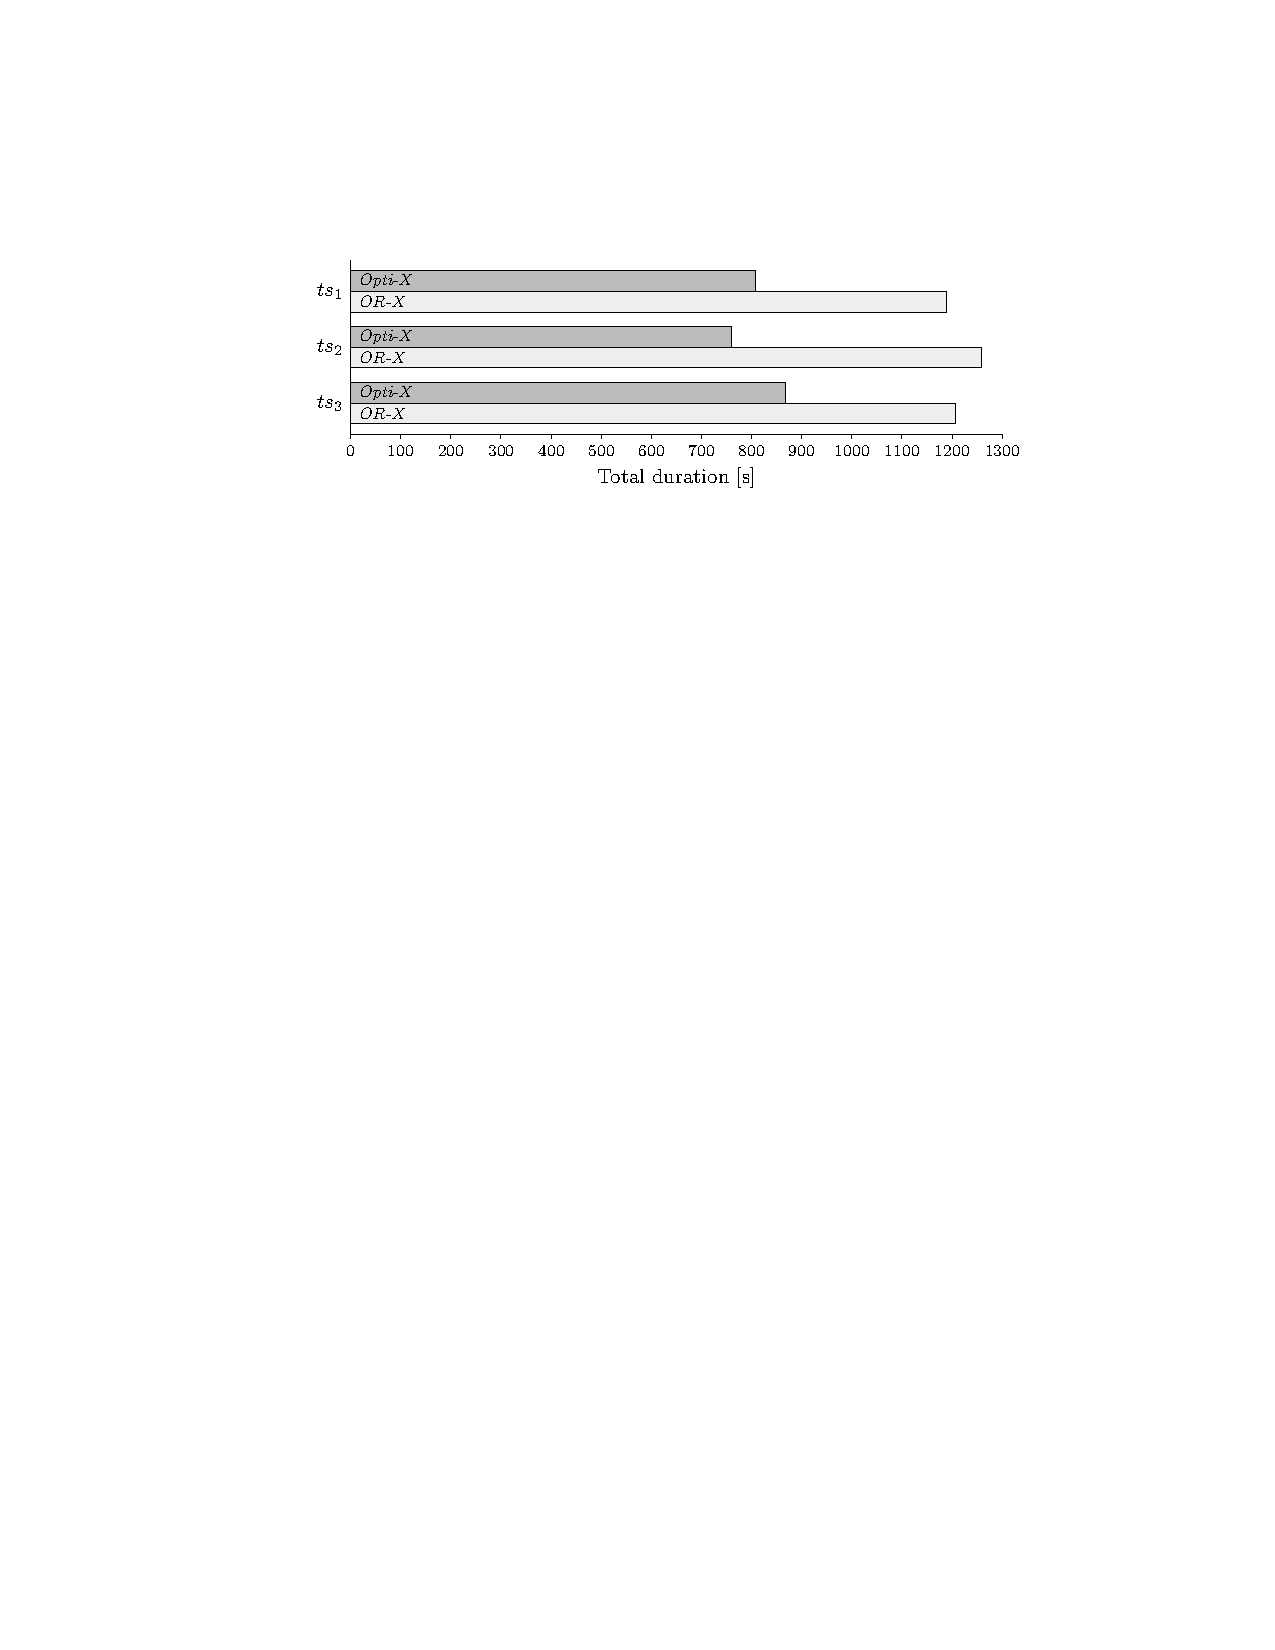
\includegraphics[width=\textwidth]{figures/test_results/1st.pdf}
    \caption{Results of Sub-Collection 1}
    \label{1st_test_set}
\end{figure}

The first sub-collection of test sets consisted of $ts_1$, $ts_2$ and $ts_3$, with 1000 tests and 100 test machines. This sub-collection was designed to test the mechanisms in situations with a large number of both tests and machines, and an abundance of possible solutions.

As can be seen from Figure \ref{1st_test_set}, Opti-X provided excellent results compared to OR-X for these test sets. Not only were all of the execution times provided by Opti-Run between 305 and 472 seconds faster than OR, it also excelled in searching time. $ts_1$ was the test set with the most possible solutions, as all tests could be executed on all machines, and thus the only test set with which Opti-X timed out after 30 seconds. Although the searching process of OR-X times out after 30 seconds, the whole process took just over 34 seconds in all of these cases, which is likely due to a combination of the large number of elements in the result list, the lock explained in Chapter \ref{chapter.implementation} not being available and the post-processing needed to extract the result. This was the sub-collection in which Opti-X was the most prominent.


\begin{figure}[t]
    \centering
    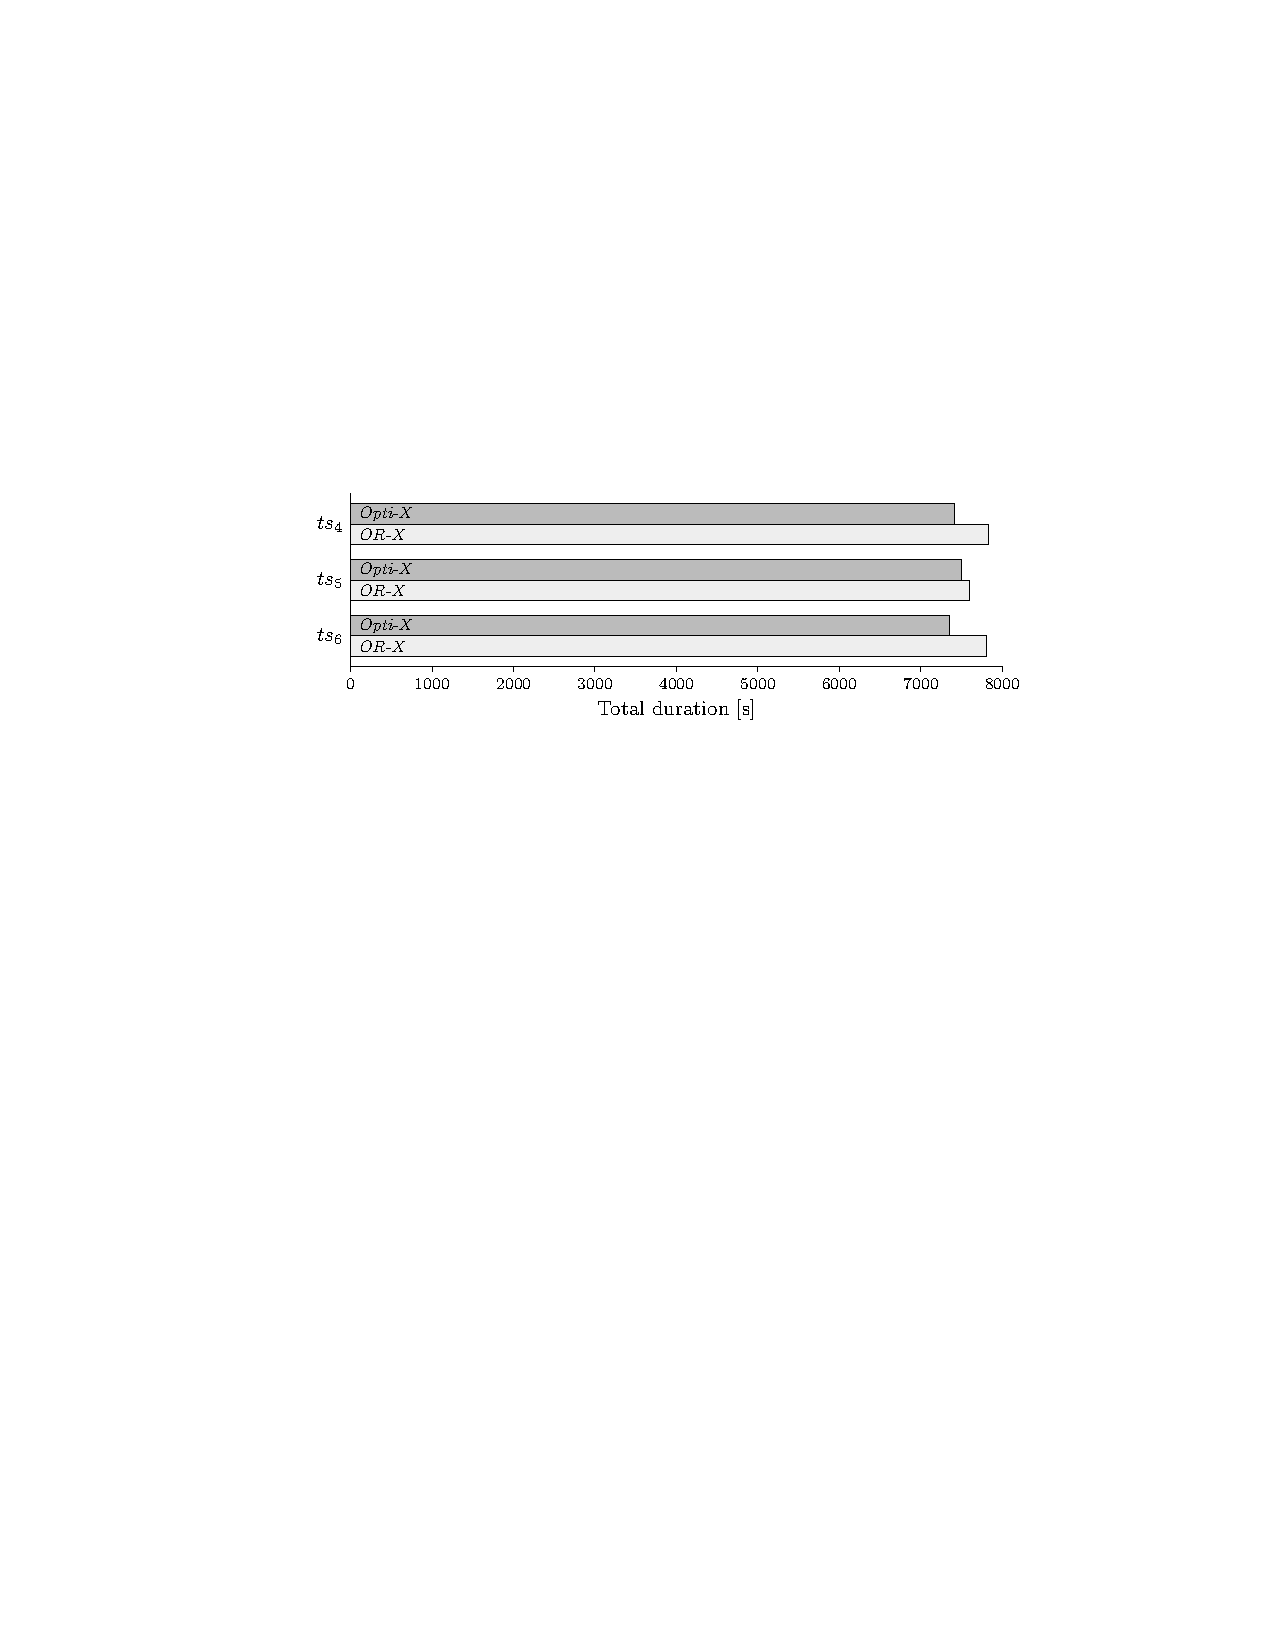
\includegraphics[width=\textwidth]{figures/test_results/2nd.pdf}
    \caption{Results of Sub-Collection 2}
    \label{2nd_test_set}
\end{figure}

The second sub-collection of test sets consisted of $ts_4$, $ts_5$ and $ts_6$, with 1000 tests and 10 test machines, and was designed to test the mechanisms in situations with a large number of tests and a small number of machines.

Figure \ref{2nd_test_set} shows that even though Opti-X provided better total time than OR-X on all test sets, the difference between the two mechanisms are less prominent in this sub-collection than in the previous one. The largest difference in total time is 449.07 seconds for $ts_6$, and the smallest 102.11 seconds for $ts_5$, which are both almost insignificant considering the total duration is more than two hours for both mechanisms on each test set in the sub-collection. This is likely linked to the much smaller number of possible solutions in the test sets in this sub-collection compared to the first one. Nevertheless, Opti-X undeniably outperformed OR-X in searching time, where Opti-X used less than a second on each test set and OR-X timed out after 30 seconds, as well as in the execution time, and thus the total time on all test sets in the sub-collection.

\begin{figure}[h!]
    \centering
    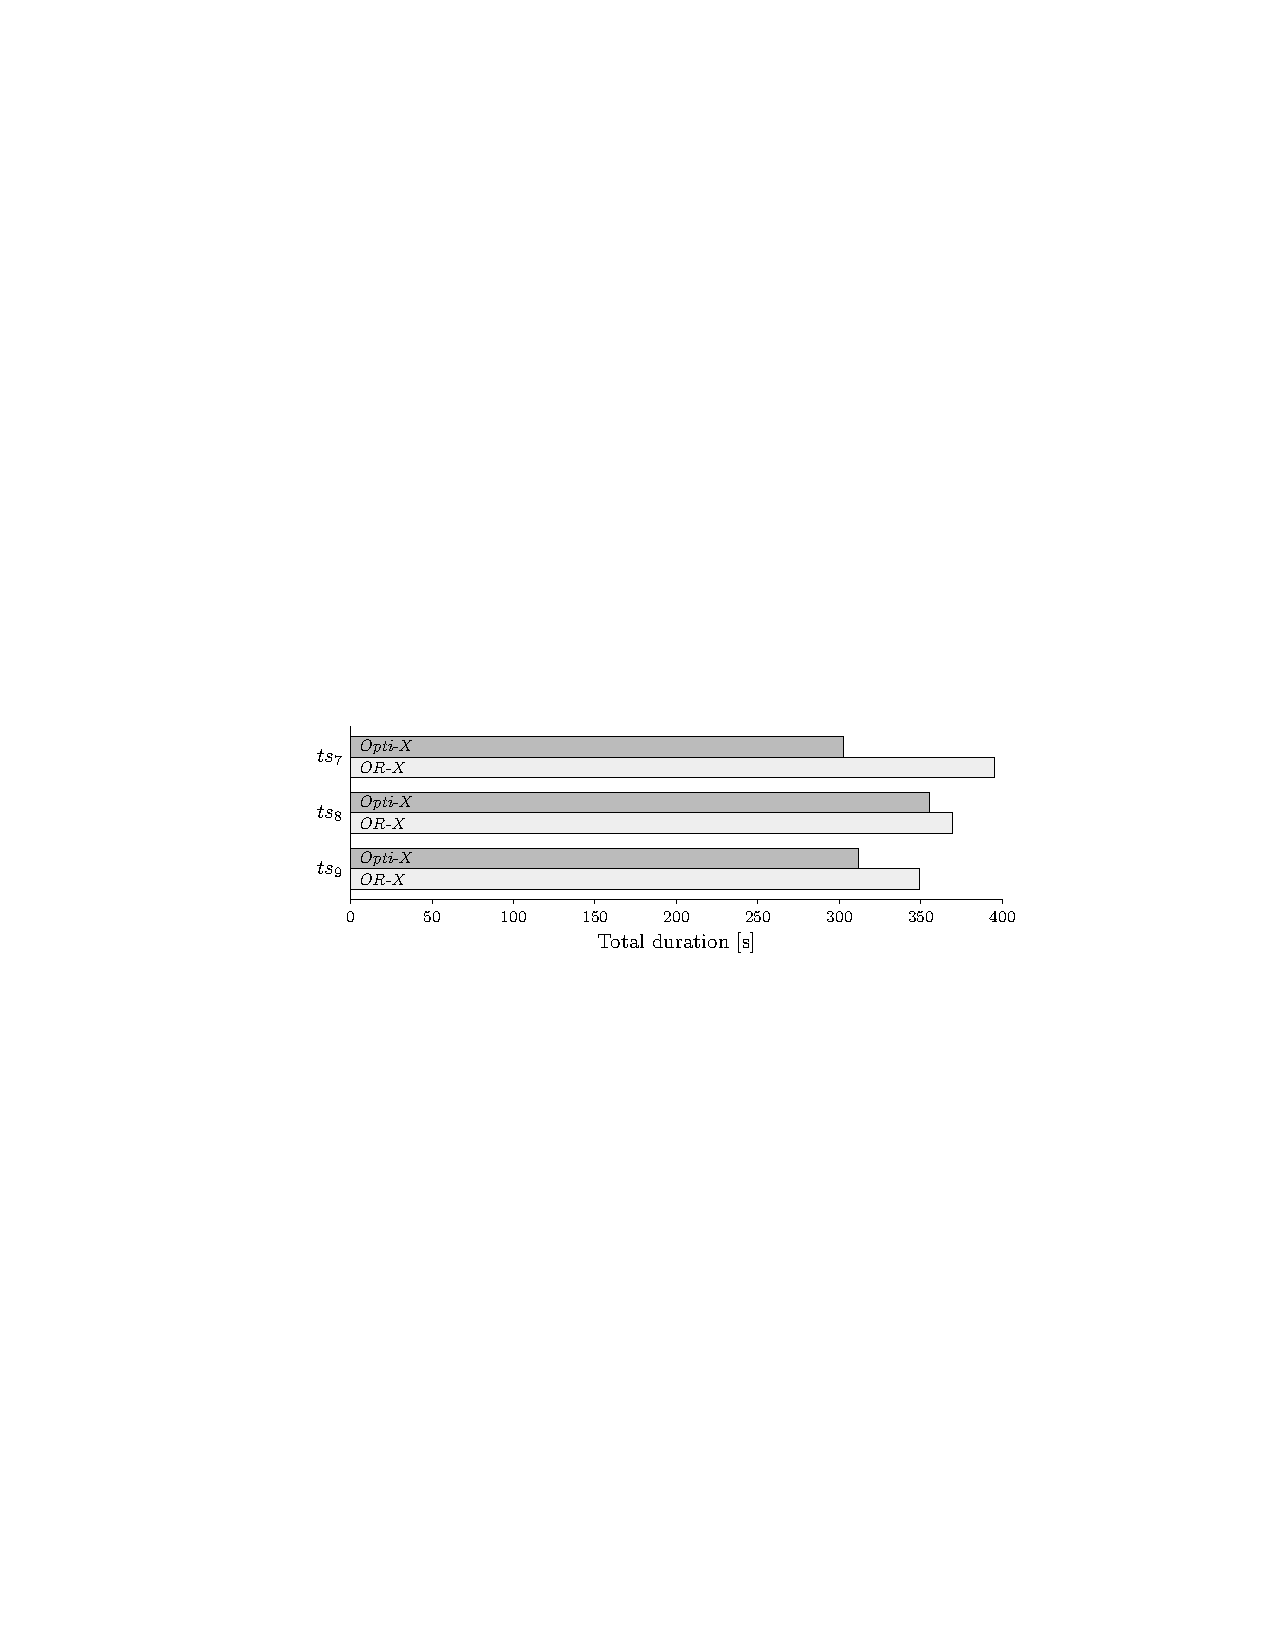
\includegraphics[width=\textwidth]{figures/test_results/3rd.pdf}
    \caption{Results of Sub-Collection 3}
    \label{3rd_test_set}
\end{figure}

The third sub-collection of test sets consisted of $ts_7$, $ts_8$ and $ts_9$, with 200 tests and 50 test machines, and was designed to test the mechanisms in situations with more realistically number of tests, and a fair number of machines.

Figure \ref{3rd_test_set} shows that Opti-X once again provided better total results for all of the test sets in the sub-collection. Opti-X finished searching after 1.72, 0.22 and 0.67 seconds respectively for the three test sets, while OR-X again was timed out after 30 seconds.

$ts_7$, which was the test set with the largest number of possible solutions, was also the one in which the difference between the two mechanisms were distinct with a total difference of 92.67 seconds. The two remaining differences were not as conspicuous, but what was interesting was that OR-X provided a 17 second shorter execution time for $ts_8$ than Opti-X accomplished. However, by using 30 seconds to find this solution, Opti-X still provided a better total time. This demonstrates that it is not enough to find an allocation in which the execution time is minimized; it is also important to minimize the time taken to find the solution. 

\begin{figure}[h]
    \centering
    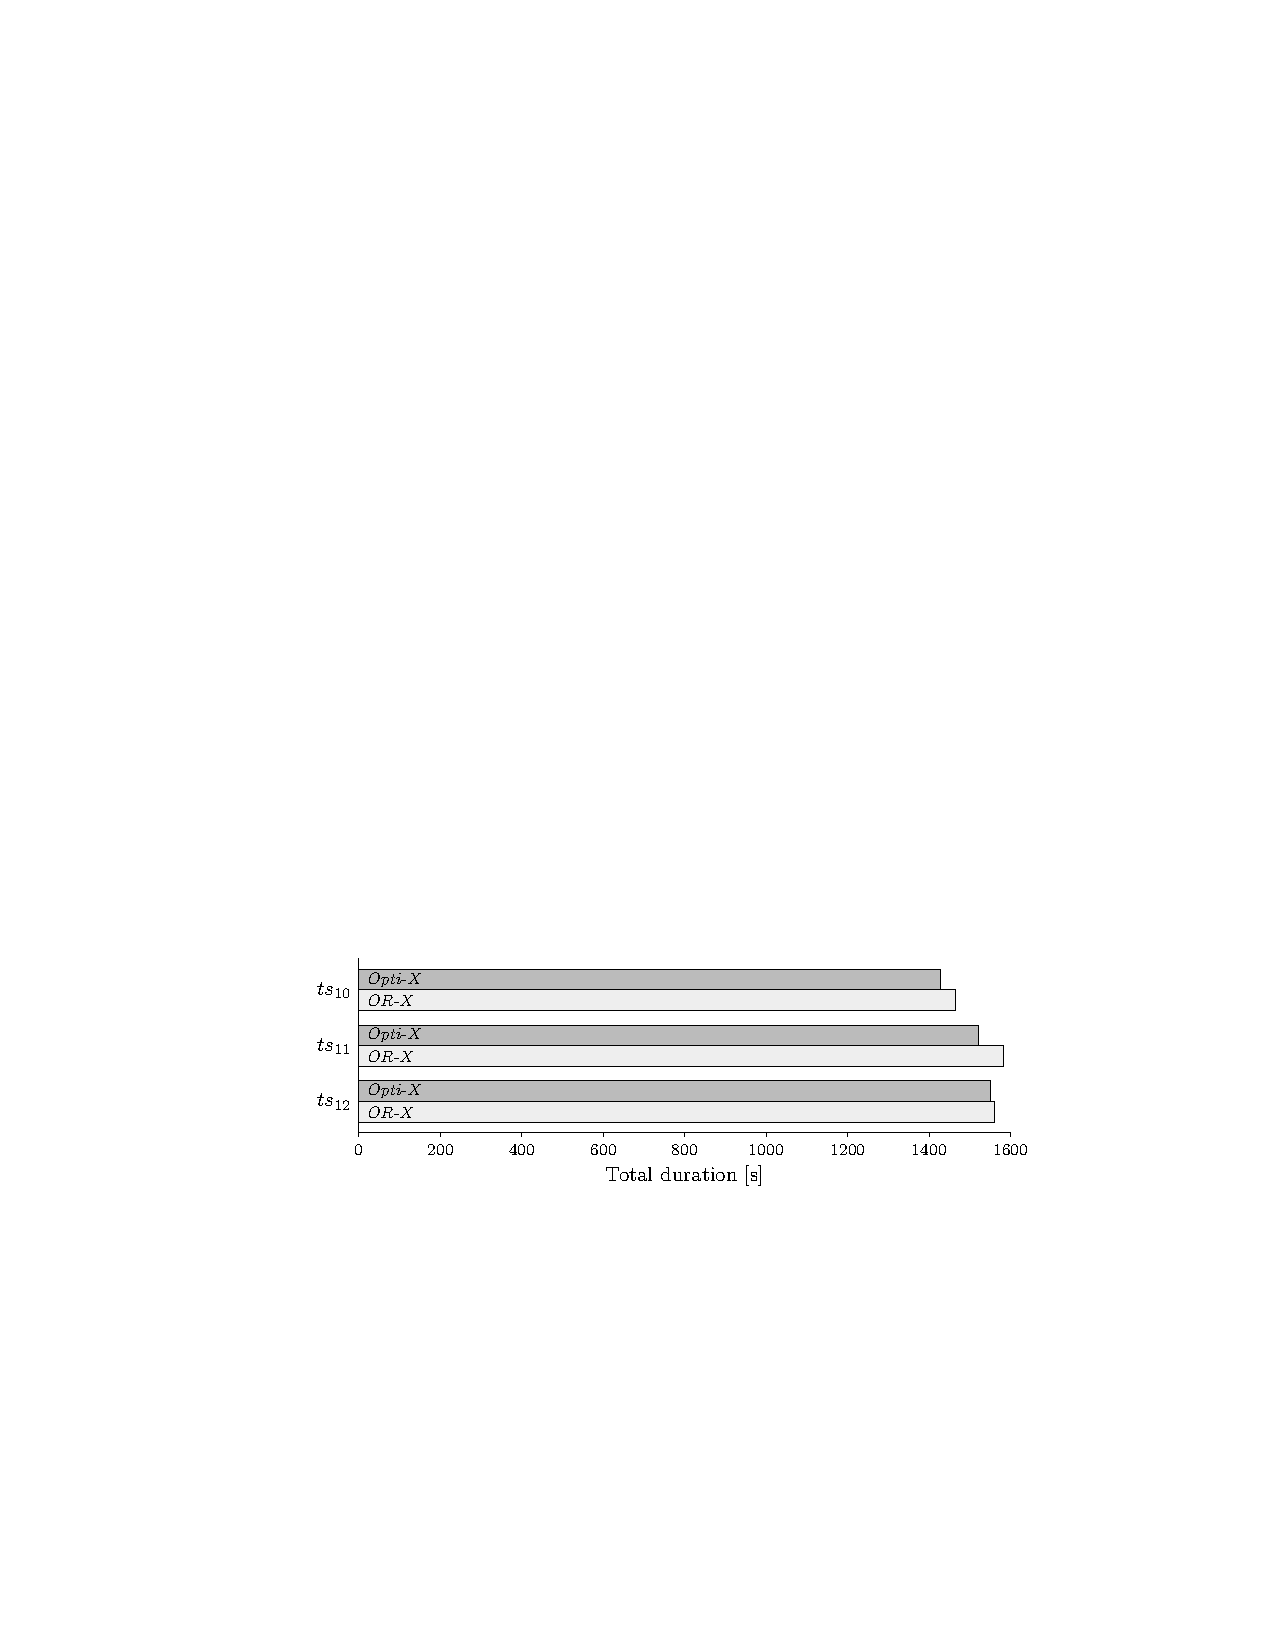
\includegraphics[width=\textwidth]{figures/test_results/4th.pdf}
    \caption{Results of Sub-Collection 4}
    \label{4th_test_set}
\end{figure}

The fourth and last sub-collection of test sets consisted of $ts_{10}$, $ts_{11}$ and $ts_{12}$, with 200 tests and 10 test machines, and was designed to test the mechanisms in situations with realistic number of both tests and machines.

Again, Opti-X produced better results for all of the test sets, which can be seen in Figure \ref{4th_test_set}. As with sub-collection 3, the differences in results were not as outstanding for this sub-collection as for the two first ones. This is likely due to a much more limited amount of possible solutions to the problem, as the number of test machines was small and the number of tests moderate.

The largest difference in execution time was a mere 33 seconds for $ts_{11}$. Again, OR-X produced a better solution of execution time for $ts_{12}$, but since Opti-X used less than a second to find its solution for this and the remaining test sets, and OR-X again was timed out after 30 seconds for the whole sub-collection, Opti-X provided the overall best result of 1549.80 seconds, which was 11.26 seconds less than the total time found by OR-X for this problem.

%\begin{center}* * *\end{center}
\begin{center}------------------------------\end{center}

\improvement{Re-formulate this entire section}

\noindent Opti-X provided better overall results than OR-X on all of the test sets in the collection. The searching time was generally exceptional, aside from for $ts_1$, where the searching was timed out after 30 seconds, and $ts_2$, where the searching time was more than 8 seconds. Compared to the searching times of OR-X, Opti-X did a better job 

Bla bla trend that OR-X uses a lot of time to find good results, and that the results found most of the time are bad compared to Opti-X. Both mechanisms were timed out upon solving the problem with the most possible solutions, but Opti-X' result was still 68\% of Or-X'.

OR-X could perhaps have provided better execution time for most, if not all, test sets if given longer time before the search timed out. However, 

Although the results provided by OR-X generally can not compete with those provided by Opti-X, the former generally produced decent results most of the time. OR-Tools is an excellent library for solving CP and combinatorial problems, but Opti-X provided better results in this specific problem. A contributing factor to this can be explained by Opti-X being designed and implemented specifically to solve this type of problem efficiently, whereas OR-Tools was designed to provide feasible solutions to a much broader range of problems. It is therefore not guaranteed to make the best decisions at any point of the process, so the time taken to identify good solutions is inclined to take more time. This is likely the reason why OR-X did not stop before the timeout of 30 seconds on any of the test sets, whereas Opti-X used less than a second on most of them.

\subsection{Threats to Validity}

Judging from the results obtained in the previous section, it is clear that Opti-X is performs superiorly compared to OR-X in the experiments. Before moving on to discussing \toolname \space as a whole, it is therefore important to establish some possible contributing factors that may threaten the validity of the results.

As explained in the previous section, the test data was randomly generated. This means that there might have been some degree of chance involved, and that if the test sets were generated again, other results may be obtained. Additionally, there might have been some interesting situations in which to test the performance of the allocation mechanisms, that are not covered in the experimental evaluation. Even though the author tried their best to come up with realistic and representative scenarios to cover the allocation mechanism in full measure, there just might have been some scenarios that did not come to mind. Also, there might be some scenarios that would provide value despite being deemed pointless to test by the author.

The results may also depend on the performance of the machine that the experiments were conducted on. Had the experiments been conducted on a newer and faster machine with better specs, the results would likely come out slightly different. OR-X would perhaps be able to reach better solutions before being timed out, and could thus possibly be a stronger competitor, whereas the results obtained by Opti-X would not likely be affected as much, as most of the problems were solved in less than a second.

Another contributing factor may be the author's knowledge of and experience with OR-Tools being far from optimal. With limited documentation and general online and literary coverage, exploring every corner of the library just could not be done with a narrow time-frame and other tasks that had to be prioritized. Although the author did invest a fair amount of time and energy in getting acquainted with the tools and tried their best to implement OR-X to be as strong of a competitor to Opti-X as possible, it may be a very real possibility that there are ways to implement it that would provide greater efficiency. Another possibility is that there are other optimization libraries that could potentially accomplish better results in this optimization problem than OR-Tools.

\subsection{Discussion}
\improvement[inline]{TODO}
\comment{A lot of good stuff and quite a lot of bad stuff.}

\subsection{Return on Investment}
\improvement[inline]{TODO}
\comment{- What is needed in order for the product to be used (Learning to set up and use the tool, dedicated machines, learning to write automated tests and learning to use optiruns template for automated tests, learning python if they don't know it already)
- Was it worth it (for Altibox)?
- How optirun competes with alternative tools
- Compare to current test process?


This chapter will include:\\
- Research questions\\
- Thorough performance comparison of optx and orx - use graphs!\\
- Evaluation of allocation mechanism\\
- Discussion of complete system\\
- Discussion of how \toolname \space can affect Altibox' overall testing process of TV Overalt (time saved or more time used to write tests? Human mistakes avoided if tests are written well, etc.). Compare to how the test process has previously been.


The existing test process will be discussed in Chapter \ref(chapter.discussion).
Test automation has previously been completely omitted, and Altibox was avid to include this in the testing of their software products.
}

